% This is "www2010-sample.tex" copied from "www2005-sample.tex" V1.2 January 26 2004
% This file should be compiled with V1.4 of "www2010-submission.class"
%
% This example file demonstrates the use of the 'www2010-submission.cls'
% V1.4 LaTeX2e document class file. It is for those submitting
% articles to the WWW'04 Conference WHO DO NOT WISH TO 
% STRICTLY ADHERE TO THE SIGS (PUBS-BOARD-ENDORSED) STYLE.
% The 'www2010-submission.cls' file will produce a similar-looking,
% albeit, 'tighter' paper resulting in, invariably, fewer pages.
%
% ----------------------------------------------------------------------------------------------------------------
% This .tex file (and associated .cls V1.4) produces:
%       1) NO Permission Statement
%       2) WWW'04-specific conference (location) information
%       3) The Copyright Line with ACM data
%       4) NO page numbers
%
% ---------------------------------------------------------------------------------------------------------------
% This .tex source is an example which *does* use
% the .bib file (from which the .bbl file % is produced).
% REMEMBER HOWEVER: After having produced the .bbl file,
% and prior to final submission, you *NEED* to 'insert'
% your .bbl file into your source .tex file so as to provide
% ONE 'self-contained' source file.
%
% ================= IF YOU HAVE QUESTIONS =======================
% Questions regarding the SIGS styles, SIGS policies and
% procedures, Conferences etc. should be sent to
% Julie Goetz (goetz@acm.org) or Adrienne Griscti (griscti@acm.org)
%
% Technical questions only to
% Gerald Murray (murray@acm.org)
% ===============================================================
%
% For tracking purposes - this is V1.2 - January 26 2004
\documentclass{www2010-submission}
\usepackage{moreverb}

\begin{document}
%
\title{QueryMed: An Intuitive Federated SPARQL Query Builder for Biomedical RDF Data}
%\subtitle{[Extended Abstract]
%\titlenote{A full version of this paper is available as
%\textit{Author's Guide to Preparing ACM SIG Proceedings Using
%\LaTeX$2_\epsilon$\ and BibTeX} at
%\texttt{www.acm.org/eaddress.htm}}}
%
% You need the command \numberofauthors to handle the "boxing"
% and alignment of the authors under the title, and to add
% a section for authors number 4 through n.
%
% Up to the first three authors are aligned under the title;
% use the \alignauthor commands below to handle those names
% and affiliations. Add names, affiliations, addresses for
% additional authors as the argument to \additionalauthors;
% these will be set for you without further effort on your
% part as the last section in the body of your article BEFORE
% References or any Appendices.

\numberofauthors{2}
%
% Put no more than the first THREE authors in the \author command

% NOTE: All authors should be on the first page. For instructions
% for more than 3 authors, see:
% http://www.acm.org/sigs/pubs/proceed/sigfaq.htm#a18

\author{
%
% The command \alignauthor (no curly braces needed) should
% precede each author name, affiliation/snail-mail address and
% e-mail address. Additionally, tag each line of
% affiliation/address with \affaddr, and tag the
%% e-mail address with \email.
\alignauthor Oshani Seneviratne\\
       \affaddr{Massachusetts Institute of Technology}\\
       \affaddr{Cambridge, MA}\\
       \affaddr{USA}\\
       \email{oshani@csail.mit.edu}
\alignauthor Rachel Sealfon\\
       \affaddr{Massachusetts Institute of Technology}\\
       \affaddr{Cambridge, MA}\\
       \affaddr{USA}\\
       \email{rsealfon@csail.mit.edu}
}
\date{15 Feb 2010}

\maketitle
\begin{abstract}
We have developed an open-source SPARQL query builder and result set visualizer for biomedical data, QueryMed, that allows end users to easily construct and run translational medicine queries across multiple data sources. QueryMed is flexible enough to allow queries relevant to a wide range of biomedical topics, runs federated queries across multiple SPARQL endpoints, and is designed to be accessible to users who do not know the structure of the underlying ontologies or the SPARQL query language. The system allows users to select the data sources that they wish to use, drawing on their specialized domain knowledge to decide the most appropriate data sources to query.  Users can add additional data sources if they are interested in querying endpoints that are not in the default list. After retrieval of the initial result set, query results can be filtered to improve their relevance. As an advanced search feature, the system also allows the user to exploit the underlying structure of the RDF data to improve query results. 
\end{abstract}

% A category with only the three required fields
\category{J.3}{Life and Medical Sciences}{Computer Applications}
\category{H.3.3}{Information Search and Retrieval}{Information Systems}

\keywords{Biomedical Ontologies, SPARQL, Query Federation, Query Building, Semantic Web, User Interfaces}

\section{Introduction}

The biomedical domain is among the early successes of the semantic web, due to the rapidity with which the biomedical community has made its data available in RDF triple stores. However, although a plethora of useful biomedical data is currently available in RDF, there is a need for easy-to use systems that do not require the end user to have knowledge of the underlying  structure of the data, and that also allow users to run federated queries on multiple SPARQL endpoints.  

For example, a physician may know her patient's personal information, symptoms, current medications, and genotype. She may wish to determine the patient's treatment plan and identify clinical trials for which the patient is eligible.  Although the physician has a single question--based on the information I have about this patient, what is the best treatment plan and set of clinical trials available?--there is no single data source that the physician can use to answer this question. The information that the physician needs must be gathered from numerous data sources such as Pubmed, DailyMed, Drugbank, LinkedCT, Diseasome,  and GO \cite{Pubmed, DailyMed, Drugbank, LinkedCT, Diseasome, GO}. Her question must be broken up into discrete pieces that can be executed individually at one data source at a time.  For example, to address her question, the physician might be interested in information on �coronary artery disease� (which she thinks is the cause of her patient�s symptoms). The information about the disease can be found in Diseasome. She might also want to know the set of drugs in DailyMed and Drugbank that can be used to treat coronary artery disease.  Information on clinical trials available for her patient can be found in LinkedCT.  Due to the large number of databases  that the physician needs to query in order to find an answer to her single question, she is likely to find useful a system that can automatically run queries over multiple data sources. Also, the physician may not know SPARQL query syntax, the location of the SPARQL endpoints, or the structure of the relevant ontologies. She is likely to want an intuitive way to query and to display the query result.  Developing intuitive ways to query multiple data sources and display results is both an important and a challenging problem.

This paper is organized as follows: Section 2 provides background information on the semantic web and its relevance for the biomedical domain. Section 3 describes our system. Section 4 discusses related work and illustrates how QueryMed differs from previous systems. Finally, section 5 outlines future work and summarizes the contributions of our system.


\section{Background}

\subsection{Biomedical Ontologies and Semantic Web}

Although most web data are not currently available in semantic web formats, the biomedical knowledge domain has been an early success of the semantic web \cite{Yip}. Many major biological and biomedical data resources, including Gene Ontology, DailyMed, LinkedCT, and Diseasome, are currently available as RDF triplestores.   Integrating biomedical data across multiple data sources and automatically extracting specific  knowledge from web resources are crucial tasks for physicians and biologists, and these semantic web resources represent valuable standardized repositories of information that can be automatically mined for biological knowledge.  The Semantic Web Health Care and Life Sciences Interest Group (HCLSIG) has been formed with the purpose of exploring the applications of the semantic web to the biomedical domain \cite{HCLSIG}.

However, although many valuable resources in the biomedical domain are available in RDF, there are a number of challenges that must be addressed in order to make such resources of maximal use to physicians, patients, and life scientists.  One challenge is constructing systems that allow end users to run intuitive queries on biomedical data.  Users of biomedical resources are likely to have extensive domain knowledge, but be unfamiliar with the SPARQL query language syntax and with the structure of biomedical ontologies. It is important to design user-friendly systems that allow these users to take advantage of the wealth of structured biological knowledge available on the semantic web.  Another central challenge is designing systems that permit users to query multiple data sources simultaneously, since relevant biological data is often distributed among many sources \cite{Pasquier}. 

\section{QueryMed}

\subsection{Architecture overview}

A general overview of QueryMed architecture is shown in Figure 1. The main components of the system are the user interface and the proxy server that retrieves biomedical data from remote SPARQL endpoints. 

QueryMed is implemented in Java in the backend and JavaScript in the frontend.  The JQuery library \cite{Resig} was used to develop an attractive user interface.  In the backend, the Jena library \cite{McBride} is used to run the SPARQL queries. QueryMed relies on the following remote resources:
\begin{itemize}
\item \textbf{SPARQL Endpoints}:  QueryMed runs queries on multiple remote SPARQL endpoints that expose biomedical data.
\item \textbf{Sources List}: The default list of endpoints available to the user is stored in a source list on the proxy server.
\end{itemize}

\begin{figure}
\centering
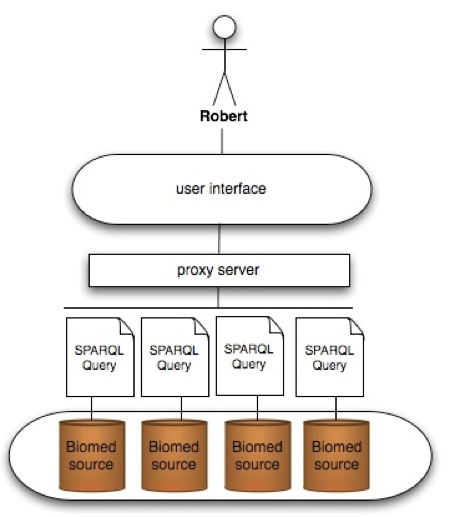
\epsfig{file=images/architecture_overview.jpg}
\caption{QueryMed Architecture Overview}
\end{figure}

\begin{figure}
\centering
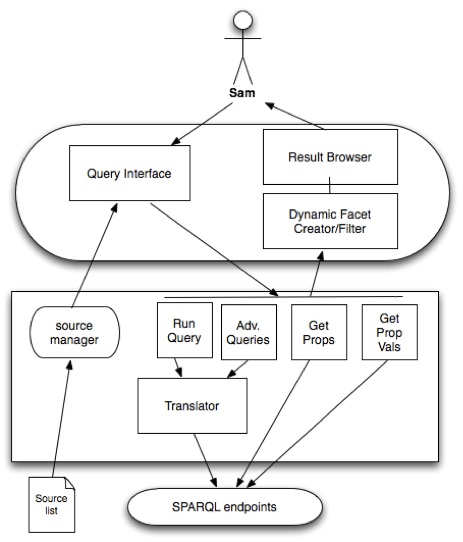
\epsfig{file=images/architecture_detail.jpg}
\caption{QueryMed Architecture details}
\end{figure}

\subsubsection{Proxy Server}

The user submits a query to the SPARQL endpoints via the proxy server.  The query is translated into a SPARQL query for each individual endpoint, and the results are returned to the user.  The specific components implemented in the proxy server are as follows.
\begin{itemize}
\item \textbf{Source Manager:} The source manager reads the source list and populates the default query list on the user interface. It also keeps track of the default endpoints, the currently selected endpoints, and the endpoints that have been dynamically added.
\item \textbf{Translator:} This component is responsible for translating the user query into valid SPARQL syntax.
\item \textbf{Run Query:} The purpose of this service is to run SPARQL queries.  It takes input on source and keyword from the client, and returns  the query results as a JSON object. The structure of the JSON object is given in figure 4.
\item \textbf{Get Properties:} This service takes as input an individual source, and returns an array of all properties for that source.
\item \textbf{Get Property Values:} This service takes as input an individual source and a specific property.  It returns a list of the possible values that this property can take.
\item \textbf{Advanced Queries:} This service takes as input list of sources, properties, query terms, and logical operators, which are passed to the proxy server as a JSON object. The structure of this JSON object is given in figure 5. After constructing and executing the SPARQL query, it returns a set of query results as a JSON object in the format given in figure 4.
\end{itemize}

\subsubsection{User Interface}

The query interface is implemented in JavaScript, HTML and CSS. The main components of the user interface are as follows: 
\begin{itemize}
\item \textbf{Initial Query Interface:} The user inputs their query  term into the provided text box (figure 6).
\item \textbf{Add New Source:} Allows the user to add a new data source to extend the query. (figure 8)
\item \textbf{Dynamic Facet Creator/Filter:} This component allows the user to select a  set of  data sources, load the properties available at these sources, and dynamically construct a complex SPARQL query connected by logical operators to take advantage of the structure of the data at each endpoint (figure 13).
\item \textbf{Result Browser:} The user can view their query results, organized by source. The results are presented in a table with pagination.  The user can choose the number of results viewed at a time, search the columns based on some text value and also sort the columns (figure 14).
\end{itemize}

\subsection{System Functionality and Design Decisions}

\subsubsection{Source list}

Because the set of default endpoints is stored on the proxy server, the set of resources available by default to the user can easily be updated.  Since useful biomedical resources are rapidly being developed and made available as RDF triple stores, the ease of updating the resource list ensures that the system can easily be brought up to date. In fact, the QueryMed system could easily be adapted to perform queries outside the biomedical domain by modifying the list of input data sources.

\subsubsection{Proxy Server}

While an entirely client side application is possible, we chose to have a proxy server perform the SPARQL query execution and caching. This design is advantageous for several reasons:
1. Efficient cache management: The result set from running an unrestricted query can include millions of results. It may be infeasible to keep unfiltered query results in browser memory. A typical memory footprint for a browser (for e.g. Firefox) is usually between 20MB and 100MB. A poorly constructed query can result in gigabytes worth of triples returned, causing the browser to crash. The proxy server can cache results from initial query execution, so that only a filtered result set is subsequently returned to the client.
2. The proxy server enables us to avoid cross domain XML-HTTP-Request errors in accessing SPARQL endpoints in various domains.


\subsubsection{Data Structures}

The parameters required for constructing the SPARQL queries are sent from the user interface to the proxy server. In the general ``Query All� case, the system will take the user-specified query term as text-box input, filter on all the triples available at the SPARQL endpoint to select only those that contain the keyword, and display the results. The generated SPARQL query will be of the form illustrated in figure 3. The word �input� in the figure represents the keyword specified by the user.


\begin{verbatimtab}
SELECT ?projection_1 ?projection_2 ... 
	?projection_n
WHERE {?x source:property ? projection 
	FILTER regex(? projection, '" + 
	input +"', 'i)
}
... //Other property filers are to follow
\end{verbatimtab}
Minimal SPARQL query structure in the �Query All� case 

When the results are returned, each result set is structured as the JSON object given in figure 4. This object identifies the endpoint where the query was executed, the URI of the endpoint, the query variables . how many results are returned and the result set.

When the user runs an advanced query, the payload to be sent to the proxy server to do the SPARQL query construction and query execution orchestration is far more complex than in the ``Query All� case. The system must specify what data sources are to be queried, what properties are queried, the values for each of the selected properties, and how these property-value pairs relate to the original user-specified query term. This information is passed as a JSON object , whose structure is given in figure 5, to the proxy server.


\begin{verbatimtab}
{
     "bindings":
     [
     	{"source" : "source_label",
     	 "uri" : "http://source.com/sparql.",
     	 "vars" : ["variable1","variable2"],
     	 "count":2,
     	 "results" : 
     		[
     		 {"variable1": "Value 1",
		  "variable1": "Value 2"},
     		 {"variable1": "Another Value 1",
		  "variable1": "Another Value 2"},
     		
     		]
     	}
     	,
	{ //Another Source and Result Description
	...
	},
	...
     ]
 }
\end{verbatimtab}
JSON returned from the RunQuery service


\begin{verbatimtab}
{
   "http://some-source/sparql": {
   	"property1": {"value1": "AND"},
	"property2": {"value 2": "OR"},
	"property2": {"value 3": "FILTER"}
	           }
	}
   //Other sources ...
}
\end{verbatimtab}
JSON constructed to send the structure of a SPARQL query for an advanced query with logical operators


\subsubsection{Query Interface}

In order to make QueryMed easy to use, but still provide a flexible tool that is able to perform a range of queries, we provide an uncluttered interface with only a  blank search box and two buttons. The ``Query All� button will perform a keyword-based query over pre-selected data sources. The advanced search option ``Refine Query� allows the user to view additional query options.  The initial query interface is shown in figure 6.

\begin{figure}
\centering
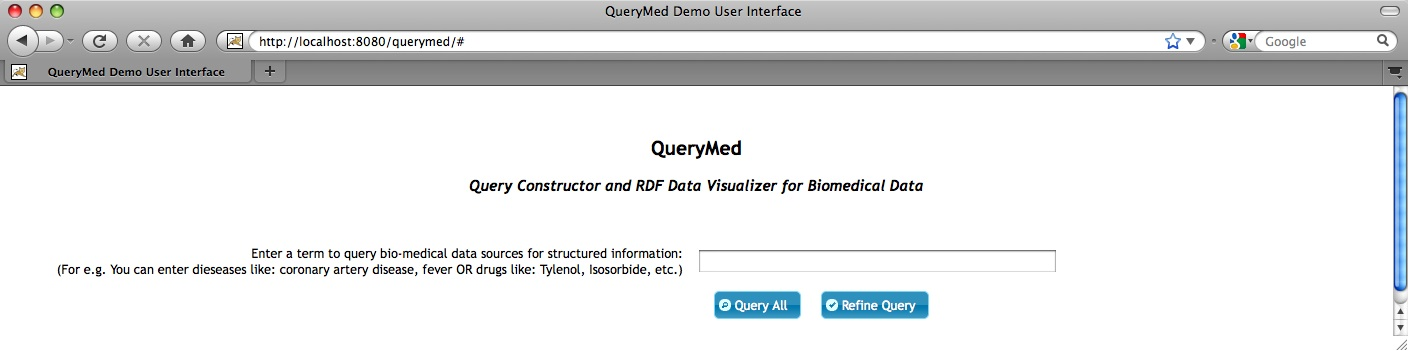
\epsfig{file=images/new_front.jpg,  width=3in}
\caption{Initial query interface seen by the user}
\end{figure}

We believe that the unstructured keyword search is likely to encourage users without previous experience running queries on semantic web data to explore the additional features of our system that allow more flexible and advanced queries.  For example, physicians who are not used to running queries on semantic web data may be more willing to invest time into learning how to find better search results once they see that the system can easily provide them with some initial useful query results using the basic keyword search option. However, the execution of queries using QueryMed will be very much different from a user issuing a web search on a search engine such as Google, because it exploits the underlying structure of the data as exposed in the individual data endpoints.

The advanced query interface provides the user with the option of selecting specific data sources to query, as shown in figure 7. The user can also dynamically add additional data sources, as shown in figure 8.  This feature allows the user to perform their query only over relevant or trusted data sources.  The ability to dynamically add additional sources increases the flexibility of  the QueryMed system, allowing users to search endpoints of interest that are not included in the default list.

\begin{figure}
\centering
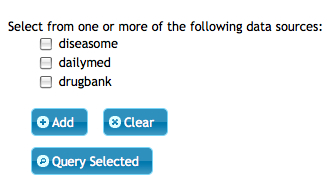
\epsfig{file=images/select.jpg,  width=3in}
\caption{The user has the option of selecting specific trusted or relevant data sources, or of adding additional data sources to query.}
\end{figure}


\begin{figure}
\centering
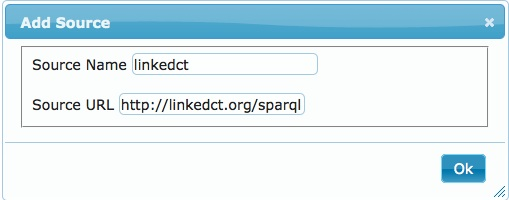
\epsfig{file=images/add_source.jpg,  width=3in}
\caption{The user can also dynamically add new data sources}
\end{figure}

When a data source is selected, the properties list is automatically populated with the properties available at the selected endpoint so that the user can run queries specific to the underlying structure of the RDF data in order to find more relevant query results. The properties list is generated by running a SPARQL query of the form given in figure 9 at the specified data source. This allows users to improve their queries using the underlying structure of the data without prior knowledge of this structure.

\begin{verbatimtab}
SELECT DISTINCT ?property
WHERE { [] ?property [] }
ORDER BY ?property
\end{verbatimtab}

Once the properties are returned, those will be displayed in the user interface as shown in figure 10. Clicking an individual property link displays a description of the property, allowing the user to understand the keywords that will be most useful to search on each specific property. A sample description for the property rdfs:label is shown in figure 11.

\begin{figure}
\centering
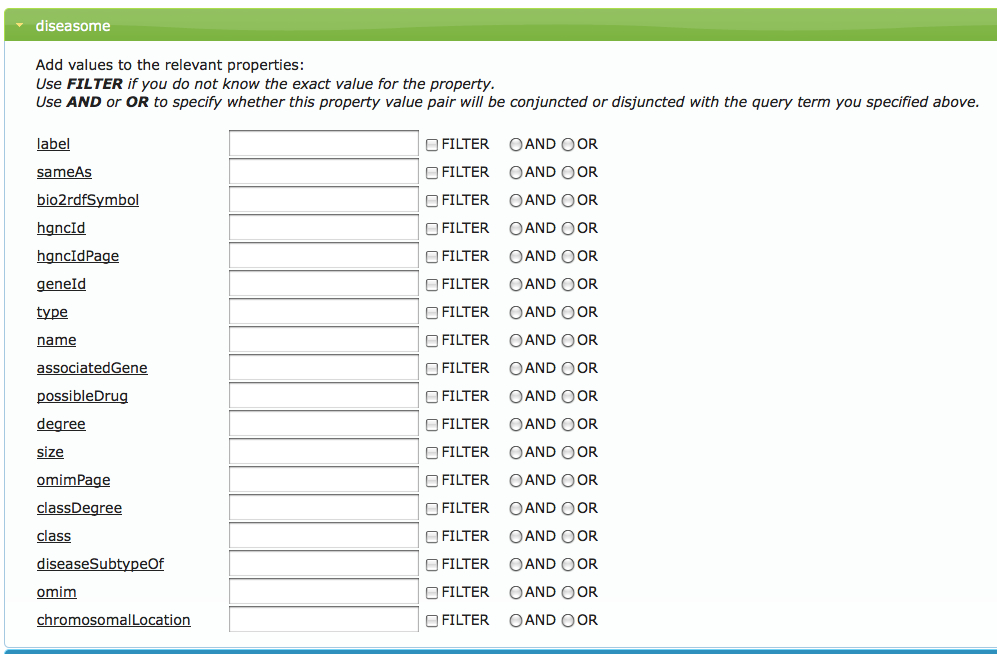
\epsfig{file=images/add_props.jpg, width=3.5in}
\caption{The Advanced Search feature allows the user to perform exact or pattern-matching queries connected by user-specified logical operators over specific properties in given resources, taking advantage of the structure in the RDF data.}
\end{figure}

The user can choose to perform exact queries, or filter results on specific keywords. If the user does not know the specific value for a property, they can instead specify a keywords using the �FILTER� option. They also can choose logical operators to connect the various parts of their query. When �AND� is used it will be appended as a basic triple pattern to the SPARQL query, i.e. as a conjunction. When �OR� is used the specified graph pattern is made to disjunct with the rest of the query with the SPARQL UNION operator. If no logical operator is specified, �AND� will be used by default.  The advanced query feature is capable of dynamically constructing complex SPARQL queries, such as the query shown in figure 12.

\begin{verbatimtab}
SELECT distinct ?disease WHERE { 
{?x <http://www.w3.org/2000/01/rdf-schema#label> 
?disease 
FILTER regex(?disease, 
"coronary artery disease", "i"). 
?x <http://www4.wiwiss.fu-berlin.de/diseasome/
resource/diseasome/class> 
<http://www4.wiwiss.fu-berlin.de/diseasome/
resource/diseaseClass/Cardiovascular>} 
UNION { ?x <http://www4.wiwiss.fu-berlin.de/
diseasome/resource/diseasome/associatedGene>
 <http://www4.wiwiss.fu-berlin.de/diseasome/
 resource/genes/ABCA1>.}
}
\end{verbatimtab}
A complex SPARQL query that takes advantage of the underlying data structure can be dynamically constructed using the advanced query feature of the QueryMed system.

The Dynamic Facet Creator shown in figure 13 allows the user to view properties from multiple endpoints, and to expand and contract properties for individual endpoints.  This feature enables the interface to display many property lists simultaneously, grouped by source, so that only information relevant to the endpoint the user is currently examining will be visible at any time.

\begin{figure}
\centering
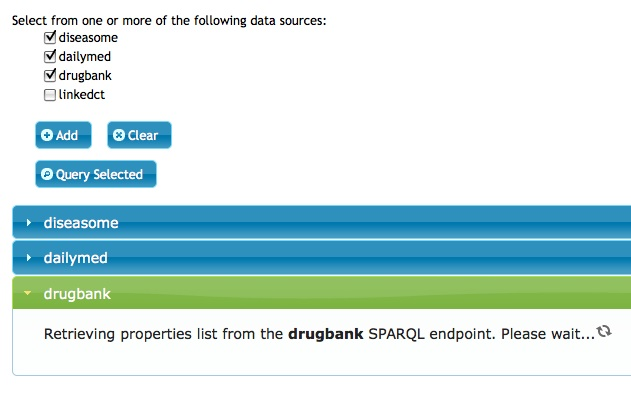
\epsfig{file=images/facet_creator.jpg, width=3in}
\caption{Dynamic Facet Creator and Filter}
\end{figure}

Query results are displayed to the user as a table, which can be filtered and searched to refine the query result, or printed as shown in in figure 14. This feature allows the user to perform additional filtering on the query results to display the most relevant results, and is particularly useful for refining queries that return a large number of results.

\begin{figure}
\centering
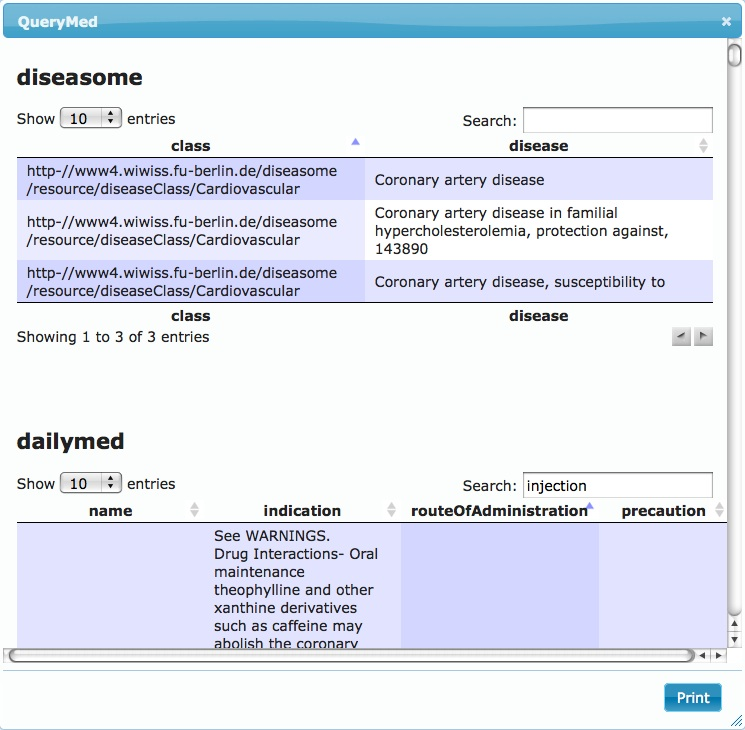
\epsfig{file=images/results.jpg, width=3.5in}
\caption{A sample result table}
\end{figure}

\subsection{Performance}

The slowest step in running queries using the QueryMed system is populating the property values for each selected endpoint.  We compared the times required to load properties from several endpoints, by running the query illustrated in figure 9.  Timing data are shown in table 2.

\begin{table}
\begin{tabular}{|l||l|l|l|}
\hline
 & Dieseasome & Dailymed & Drugbank \\
\hline
\hline
1st Trial   & 3.45 s & 1.77 s  & 9.51 s  \\
2nd Trial  & 1.61 s & 1.57 s & 9.34 s \\
3rf Trial  & 1.71 s & 1.66 s & 9.06 s \\
\hline
\end{tabular}
\caption{Running times to retrieve all the properties from selected endpoints}
\end{table}


For all selected endpoints, the property values take longer to load on the initial query than in subsequent iterations, probably due to browser caching. The running time to acquire the list of property values for the Drugbank endpoint is much larger than the time for the other two endpoints, probably due to the greater size of the Drugbank database.  (As of 12/10/09, Diseasome contains 91,182 triples, DailyMed contains 164,276 triples, and DrugBank contains 765,936 triples).

\subsection{QueryMed Resources}

The source code for the Querymed system is available at the QueryMed Google Code project: \\
http://code.google.com/p/querymed/

A video displaying a sample use case can be found at: \\
http://www.youtube.com/watch?v=JCr7vryS9Vg 

\section{Related Work}

A number of existing tools aim to provide a user-friendly interface for browsing semantic web data, or to allow users to perform federated queries.  Several of these are described below.

The SMART query tool is a web-based application designed to allow biologists to run SPARQL queries over multiple endpoints.  Queries to the SMART system are constructed using a descriptive logic query written in the natural-language like Manchester OWL syntax \cite{Battista}.  However, it cannot be expected that the end users know how  to use the Manchester OWL syntax to write queries, whereas in QueryMed, users can construct queries intuitively by giving keywords for user selected properties. 

GoWeb is another system designed for answering queries on biomedical data. It allows users to run traditional keyword-based web search with ontology search features \cite{Dietze}. After a keyword search, documents can be filtered based on the biomedical annotations they contain. However, in GoWeb the exact sources queried are not transparent and cannot be selected or modified by the user as in QueryMed.

Twinkle offers a stand-alone graphical user interface to load and edit SPARQL queries that can be used to query online SPARQL endpoints \cite{Dodds}. Our system differs from the Twinkle system in several aspects. First of all, in Twinkle, the user is expected to know what is already available at the SPARQL endpoints to write the query. But in QueryMed, we only ask for specific keywords of interest, and give the option of restricting the query should the user wish to run a more precise query. Second, although Twinkle was designed to be a more general purpose system, it only supports a small number of specific SPARQL endpoints, while QueryMed allows the user to dynamically add SPARQL endpoints.

Most SPARQL query engines are designed to run queries against individual endpoints. But it is often useful to draw on multiple web resources in answering a query. There are a number of systems, including the DARQ \cite{Quilitz} and CALO query manager \cite{Ambrite}systems, designed to allow the user to run integrated queries against multiple SPARQL endpoints. 

\begin{table*}
\begin{center}
\begin{tabular}{| p{2cm} | p{2cm}| p{2cm}| p{2cm}| p{2cm}| p{2cm} |}
\hline
 & Query Multiple Sources? & Dynamic Addition of Sources & Allows Keyword Queries & Open Source & GUI \\
\hline
\hline
QueryMed  & Yes & Yes & Yes & Yes & Yes  \\
\hline
SMART  & Yes & No & No & Yes & Yes  \\
\hline
DARQ  & Yes & N/A & No & Yes & No  \\
\hline
GoWeb  & Yes & No & Yes & No & Yes  \\
\hline
BioGateway  & Yes & No & No & No & Yes  \\
\hline
Twinkle  & Yes & No & No & Yes & Yes  \\
\hline
\end{tabular}
\caption{Comparison of selected features of the QueryMed system with other related systems.}
\end{center}
\end{table*}

Table 3 compares selected features of the QueryMed system with other related systems. The QueryMed system was unique among the systems that we found in that it allows endpoints to be dynamically added by the user.  Other features of the QueryMed system that distinguished it from similar systems included the ability both to perform keyword queries and to construct more advanced queries taking advantage of the structure of the semantic web data.  This feature increases the ease of use of our system relative to other similar systems.  Furthermore, the Javascript based user interface of the QueryMed system, implemented using the JQuery library, makes our user interface particularly attractive, easy to interact with, and capable of handling a variety of user input events.  Another unique feature of our system is the property-based advanced query interface. This enables users to take advantage of the structure of the underlying ontologies used to represent the data without prior knowledge of the ontology structures. 

\section{Future Work and Conclusions}

The bottleneck in the running time of our system is running queries that must retrieve many triples from slow remote SPARQL endpoints. By caching relevant data locally, the running time could be significantly improved. We observed that the QueryMed system performs significantly faster the second time that a query is run on a given resource possibly due to browser caching. By managing our own cache to contain the data most likely to be needed on the proxy server, we could reduce running time still further. Another approach that could reduce running time still further, especially for users with a slow network connection, would be to create a complementary standalone application that gives the user the option at startup time of loading all the required RDF data. Since data is stored locally after the initial startup, using the system in subsequent queries will be rapid after an initial loading phase.  This approach might be too memory-intensive if the user wishes to run queries over many large triple stores, but might work best in the situation where there is a small or moderate amount of data in the repositories of interest to the user. 

Our system currently allows only a restricted set of SPARQL queries. Supporting additional types of queries and including query optimization functionality could increase both the flexibility and speed of the QueryMed system. By drawing on the expressivity of the SPARQL language and the information contained in the ontologies used to represent the data, it would be possible to extend our system into an intelligent reasoning system on biomedical data which allows physicians to enter sophisticated, complex queries and find relevant biomedical results.

We also believe that it would be useful to allow exploration of the relationships among multiple data sources containing similar resources.  One challenge in integrating biomedical data across multiple data sources is that individual data items (i.e, a specific protein or a specific drug) may be represented by distinct URIs at different endpoints. The diversity of representations of identical data items across different biomedical data sources makes it difficult to automatically combine these items.  However, there is some cross-referencing between the biomedical data sources that we examined (for example, DailyMed drugs sometimes refer to diseases in the Diseasome SPARQL endpoint by their URI).  It might be useful to provide a representation of the relationships among search results from different sources with the query results. Additionally, the system could automatically detect similar data items even if they are identified by distinct URIs, and group similar items from distinct data sources together in the query results by natural language processing.  Another useful feature might be to allow the user to view the relationships among distinct URIs (as in the relfinder system \cite{Heim} , which displays possible paths through the RDF graph between distinct resources).

Another feature that we have begun to implement in our system is an autocompletion feature to automatically retrieve the distinct values for any given property. This feature will allow the user to automatically see all valid choices for each property, and will make the system easier to use and reduce empty query result sets.

Since a major goal of QueryMed is ease of use by physicians, life scientists, and patients, we also plan to perform a user study to understand how effectively  users without knowledge of SPARQL can interact with our system.  We plan to use data from this study to further refine our system to improve its usability.

The main contributions of our system are: dynamic construction of complex SPARQL queries based on intuitive user input; dynamic addition of user-specified endpoints; and ability to run queries over multiple endpoints. Because of the unique features of our system, we believe it will be of use to the biomedical community.

\section{Acknowledgments}

\bibliographystyle{abbrv}
\bibliography{references}  

\end{document}
